% UMI Arena (CoRL 2026) poster, 48 x 36 in landscape. Build: latexmk -pdf poster.tex
\documentclass[final]{beamer}
\usepackage[orientation=landscape,size=custom,width=121.92,height=91.44,scale=1.3]{beamerposter}
\usepackage[T1]{fontenc}\usepackage[scaled=0.95]{helvet}\renewcommand{\familydefault}{\sfdefault}
\usepackage{booktabs,siunitx,qrcode,tikz,graphicx,ragged2e,colortbl}
\graphicspath{{../fig/}}

% ---------- theme ----------
\definecolor{ink}{HTML}{1E2A38}
\definecolor{navy}{HTML}{16324F}
\definecolor{teal}{HTML}{2A7F8F}
\definecolor{amber}{HTML}{D9822B}
\definecolor{paper}{HTML}{FBFAF7}
\definecolor{panel}{HTML}{FFFFFF}
\definecolor{muted}{HTML}{5C6670}
\setbeamertemplate{navigation symbols}{}
\setbeamercolor{background canvas}{bg=paper}
\setbeamercolor{normal text}{fg=ink}
\setbeamercolor{block title}{fg=navy,bg=panel}
\setbeamercolor{block body}{fg=ink,bg=panel}
\setbeamerfont{block title}{size=\Large,series=\bfseries}
\setbeamertemplate{block begin}{%
  \begin{beamercolorbox}[colsep*=0.4ex,dp=0.6ex,leftskip=1.2em,rightskip=1.2em]{block title}%
    \usebeamerfont{block title}\insertblocktitle\par
    \vskip-0.4ex\textcolor{teal}{\rule{\bw}{2.5pt}}%
  \end{beamercolorbox}%
  \begin{beamercolorbox}[colsep*=0.4ex,vmode,leftskip=1.2em,rightskip=1.2em]{block body}\RaggedRight}
\setbeamertemplate{block end}{\vskip0.8ex\end{beamercolorbox}\vskip1.4ex}
\setbeamertemplate{itemize item}{\color{teal}\raisebox{0.15ex}{\rule{0.55em}{0.55em}}}
\setlength{\parskip}{0.7ex}
\setlength{\leftmargini}{1.4em}
\newcommand{\bw}{\dimexpr\linewidth-2.4em\relax}
\newcommand{\key}[1]{\textbf{\color{navy}#1}}
\newcommand{\bignum}[2]{\begin{minipage}[t]{#1}\centering{\fontsize{66}{70}\selectfont\bfseries\color{amber}#2}\end{minipage}}
\newcommand{\numlabel}[2]{\begin{minipage}[t]{#1}\centering\small\color{muted}#2\end{minipage}}
\newcommand{\capt}[1]{{\small\color{muted}#1\par}}

\begin{document}
\begin{frame}[t]
\vspace*{-1.4cm}
% ---------- header ----------
\begin{tikzpicture}[overlay,remember picture]
  \fill[navy] (current page.north west) rectangle ([yshift=-12.0cm]current page.north east);
\end{tikzpicture}
\noindent\parbox[t][10.0cm][c]{\paperwidth}{%
\begin{columns}[c,totalwidth=\paperwidth]
\begin{column}{0.86\paperwidth}
  \hspace*{2.4cm}\begin{minipage}{0.95\linewidth}
  {\fontsize{76}{82}\selectfont\bfseries\color{white}A Head Camera Is (Almost) All You Need\par}
  \vspace{0.5cm}
  {\fontsize{40}{46}\selectfont\color{white!85!navy}An electronics-free UMI glove labelled and observed by one moving camera\par}
  \vspace{0.8cm}
  {\fontsize{32}{36}\selectfont\color{white}Yosub Shin$^{1}$ \quad Yuan Liu$^{2}$ \quad Igor Molybog$^{1}$\hspace{2.5cm}
   {\fontsize{26}{30}\selectfont\color{white!80!navy}$^1$University of Hawai\textquotesingle i at M\=anoa \quad $^2$Independent}\par}
  \end{minipage}
\end{column}
\begin{column}{0.14\paperwidth}
  \centering
  \colorbox{white}{\qrcode[height=7.8cm]{https://arxiv.org/abs/2610.27622}}\par
  \vspace{0.3cm}{\small\color{white}arXiv:2610.27622}\par{\small\color{white!80!navy}The UMI Arena, CoRL 2026}
\end{column}
\end{columns}}
\vspace{0.5cm}

% ---------- body ----------
\begin{columns}[t,totalwidth=0.975\paperwidth]

% ===== left two thirds =====
\begin{column}{0.655\linewidth}

\begin{block}{One camera, two mounts}
  \centering
  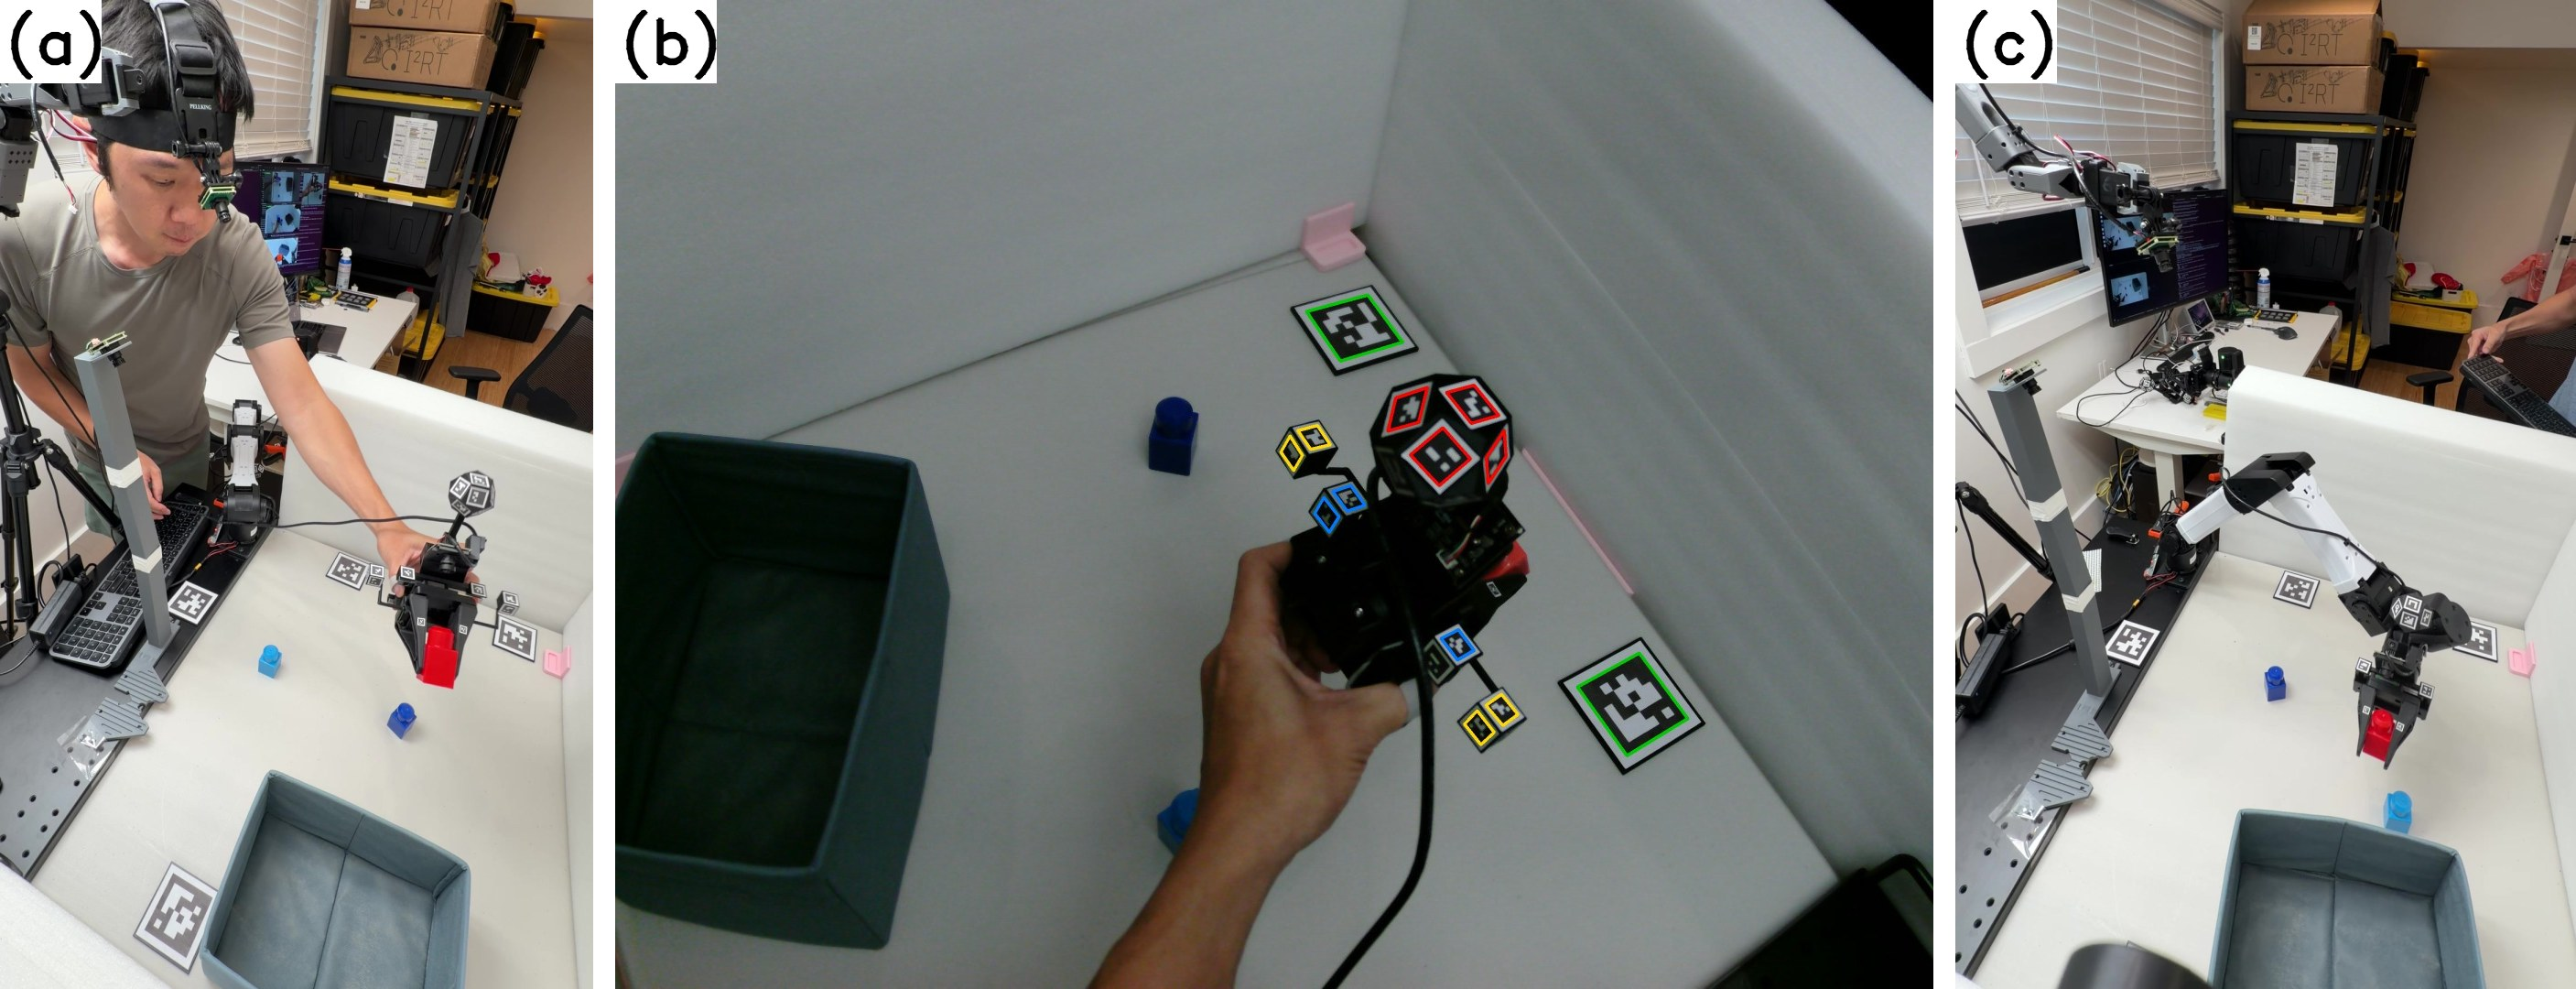
\includegraphics[width=\bw]{teaser.jpg}\par
  \vspace{0.4ex}
  \begin{minipage}{\bw}\capt{(a) A \$122 4K head camera, a \$22 electronics-free glove, four paper tiles.
  (b) The camera's own frame: tiles give the camera pose, the ball the gripper pose, the jaw tags the opening.
  (c) At deployment the same camera rides a \$122 arm beside the robot.}\end{minipage}
\end{block}

\begin{columns}[t,totalwidth=\linewidth]
\begin{column}{0.325\linewidth}
\begin{block}{Why the head}
  \begin{itemize}
    \item Wrist devices need a \key{second stream} to track the gripper: SLAM, an IMU, a controller or an external camera.
    \item \key{Gaze leads the hand}: the gripper stays in view, at arm's length, with the goal.
    \item The frames the policy sees are the frames that \key{carry the labels}.
  \end{itemize}
  No SLAM, no IMU, no wrist camera, no cables.
\end{block}
\end{column}

\begin{column}{0.325\linewidth}
\begin{block}{Labels from one frame}
  \begin{itemize}
    \item \key{Camera pose} from the paper tiles, refit from the footage to \SI{0.5}{px}.
    \item \key{Gripper pose} by PnP on a \SI{15}{mm} ArUco dodecahedron.
    \item \key{Jaw width} from printed tails on the jaws.
  \end{itemize}
  \vspace{0.3ex}
  \begin{center}
  \bignum{0.31\linewidth}{6.5\,mm}\bignum{0.31\linewidth}{1.6\textdegree}\bignum{0.34\linewidth}{3.5\,\%}\\[0.3ex]
  \numlabel{0.31\linewidth}{tool point}\numlabel{0.31\linewidth}{orientation}\numlabel{0.34\linewidth}{jaw width, of stroke}
  \end{center}
  \capt{Median error against the robot's encoders. A label on 93--100\,\% of frames.}
\end{block}
\end{column}

\begin{column}{0.325\linewidth}
\begin{block}{The robot's head}
  \begin{itemize}
    \item A \$122 six-joint arm carries the same camera beside the YAM.
    \item It follows the gripper \key{from the robot's encoders alone}, in teleoperation and in rollouts.
  \end{itemize}
  \vspace{0.3ex}
  \begin{center}
  \bignum{0.48\linewidth}{46\,mm}\bignum{0.48\linewidth}{5.4\textdegree}\\[0.3ex]
  \numlabel{0.48\linewidth}{head pose vs the collector}\numlabel{0.48\linewidth}{static camera: \SI{87}{mm}, \SI{7.0}{\degree}}
  \end{center}
\end{block}
\end{column}
\end{columns}

\begin{columns}[t,totalwidth=\linewidth]
\begin{column}{0.6\linewidth}
\begin{block}{One placement, two views}
  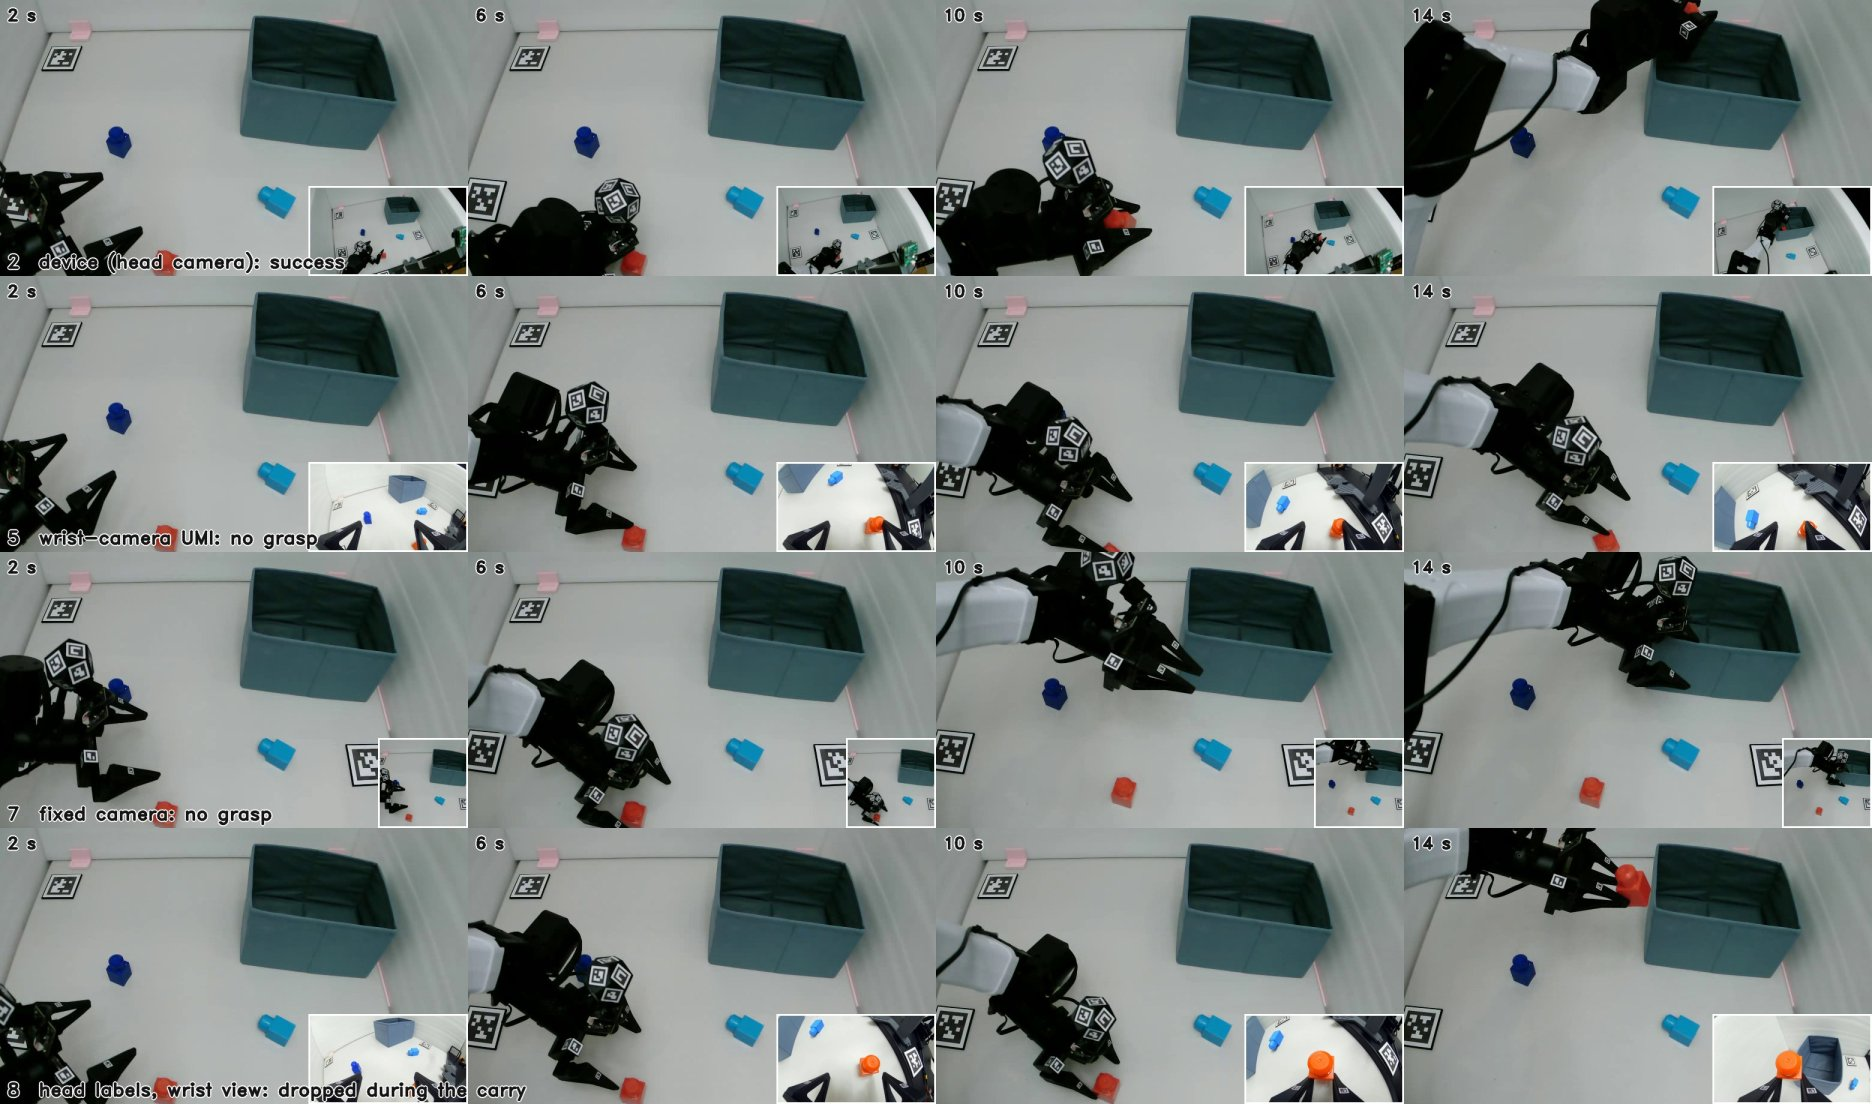
\includegraphics[width=\bw,trim=0 552bp 0 0,clip]{rollouts.jpg}\par
  \capt{Scene 16 at 2, 6, 10 and 14\,s, each policy's own view inset. Top: the head-camera policy keeps gripper and bin in one frame. Bottom: the wrist policy sees the block and the wall, and drops it.}
\end{block}
\end{column}
\begin{column}{0.4\linewidth}
\begin{block}{Collection}
  \begin{center}
  \bignum{0.48\linewidth}{\$144}\bignum{0.48\linewidth}{103\,g}\\[0.3ex]
  \numlabel{0.48\linewidth}{glove, camera, strap}\numlabel{0.48\linewidth}{on the head}\\[1.2ex]
  \bignum{0.48\linewidth}{2--3$\times$}\bignum{0.48\linewidth}{198}\\[0.3ex]
  \numlabel{0.48\linewidth}{demos per minute vs teleop}\numlabel{0.48\linewidth}{demos in four sessions}
  \end{center}
\end{block}
\end{column}
\end{columns}

\end{column}

% ===== right third: results =====
\begin{column}{0.335\linewidth}

\begin{block}{Eight policies, one recipe}
  \capt{ACT, joint-space actions, same 194 glove demos in every mix. 25 placements, one trial each.}
  \vspace{0.3ex}
  \begin{center}\normalsize
  \setlength{\tabcolsep}{6pt}\renewcommand{\arraystretch}{1.15}
  \begin{tabular}{@{}clcc@{}}
    \toprule
    \# & Policy (glove labels $\to$ observation) & Val & Success \\
    \midrule
    1 & teleop only, 172 ep.\ $\to$ head cam & 0.318 & 18/25 \\
    \rowcolor{amber!15}
    2 & \textbf{device}: head $\to$ head, 172\,+\,194 & \textbf{0.263} & \textbf{20/25} \\
    3 & teleop only, 48 ep.\ $\to$ head cam & 0.464 & 10/25 \\
    \rowcolor{amber!15}
    4 & \textbf{device, low budget}, 48\,+\,194 & 0.295 & \textbf{17/25} \\
    5 & wrist UMI: fixed $\to$ wrist fisheye & 0.257 & 15/25 \\
    6 & head-cam labels for encoders & 0.328 & 15/25 \\
    7 & fixed camera as the system & 0.256 & 12/25 \\
    8 & head labels $\to$ wrist fisheye & 0.252 & 14/25 \\
    \bottomrule
  \end{tabular}
  \end{center}
\end{block}

\begin{block}{The view decides how a policy fails}
  \begin{center}
  \bignum{0.3\linewidth}{20/25}\bignum{0.3\linewidth}{15/25}\bignum{0.3\linewidth}{12/25}\\[0.3ex]
  \numlabel{0.3\linewidth}{head camera}\numlabel{0.3\linewidth}{wrist fisheye (UMI)}\numlabel{0.3\linewidth}{fixed camera}
  \end{center}
  \vspace{0.5ex}
  \begin{itemize}
    \item Wrist policies \key{drop the block mid-carry} (12 of 21 failures), always while looking away from the bin. Head policies: 1 of 45.
    \item Same labels, other view (arms 8 vs 2): 20/25 falls to 14/25. Same view, other labels (8 vs 5): no difference.
    \item \key{Head-camera labels} cost 3\,\% of validation loss against encoders, nothing on the robot (6 vs 1).
  \end{itemize}
\end{block}

\begin{block}{194 glove demos $\approx$ 65--100 teleoperated episodes}
  \begin{center}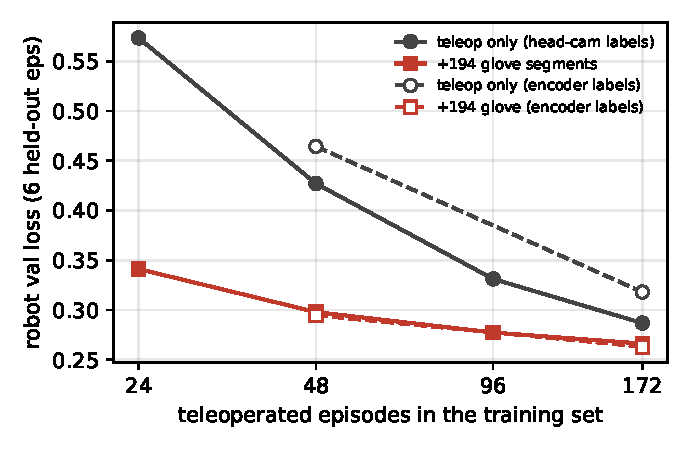
\includegraphics[width=0.86\linewidth]{budget.pdf}\end{center}
  \vspace{-0.5ex}
  \capt{Robot validation loss against teleoperation budget, with (dashed) and without the glove set. Added to 48 teleoperated episodes: 10/25 to 17/25, level with 172 alone.}
\end{block}


\begin{block}{Limits and next}
  One task, one collector, one tile layout. Glove-only policies do not transfer: co-training is required. Next: bimanual, tile-free in the wild.
\end{block}
\end{column}
\end{columns}
\end{frame}
\end{document}
